\subsubsection{Implementation}

To adapt the iterative implementation to use OpenMP, we only needed to add the following pragma to the middle for loop in the main FFT body:

\begin{lstlisting}
  #pragma omp parallel for schedule(guided)
  for(int k = 0; k < i/2; k++) {
\end{lstlisting}

This pragma defines a parallel section and tells OpenMP to split the iterations of the following for loop up for all encountering threads. The schedule clause determines in which way the loop will be split.
We tried 3 different schedule options (static, dynamic, guided) from which guided was the one that led to the best performance (closely followed by static scheduling). With this clause the first encountering thread
gets a chunk of the whole iteration space proportional to the amount of threads, each following thread gets a chunk of the remaining iteration space, again proportional to the number of threads. The schedule clause can also take
another paramter called the chunk size, which specifies the minimum size for the chunks. The default value for guided scheduling is approximately loopcount/number\_of\_threads, which is what we use in our implementation.

\subsubsection{Performance}

We did 100 repetitions and took the median as 'average' speedup, since some testcases sometimes completely destroyed the result. Further more the median wasn't always that far apart from the minimum.\newline 
Average speedup:

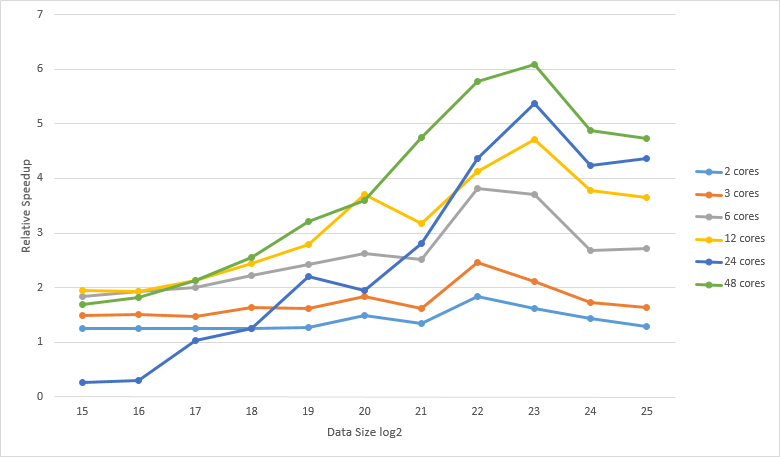
\includegraphics[width=\textwidth]{omp_it_avg.png}

\pagebreak
Best observered speedup:

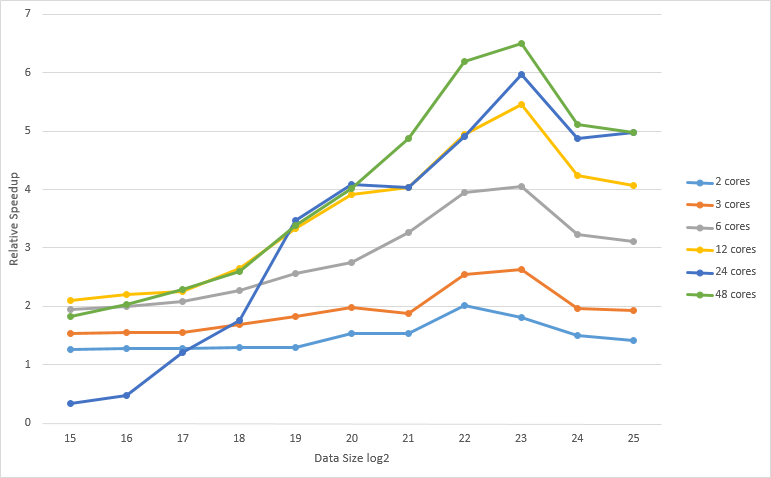
\includegraphics[width=\textwidth]{omp_it_best.png}

As expected we see the same kind of speedup curve as for the recursive implementation, but with the speedup not quite reaching the same values. Probable causes for this could be possibly higher overhead associated with the scheduling, as well as the different memory access pattern,
but we could not determine the actual cause with certainty.
